\section{Experimental Setup}
\label{sec:experiment}
%
In this section, we present the setup of the experiments to evaluate
the effectiveness of \tool{}. We address the following research
questions (RQs):

\sw{We may miss a RQ for the test results using \tool. In the setup,
  we have not said which sentiment analysis models we tested, and how
  we measure the results (e.g., number of misclassified test cases).}

\begin{enumerate}[label=\textbf{RQ\arabic*}]
\item \label{rq:one}: Can \tool generate consistent test sentence and
  its oracle?
\item \label{rq:two}: Are \tool generated test cases relevant to be used
  for their \lc evaluation?
\item \label{rq:three}: Can \tool generate more diverse test cases
  than \Cklst?
\item \label{rq:four}: Can \tool be useful to find root causes of bugs
  in the \sa models?
%% \item \label{rq:three}: How effective is our new test case generation
%%   using \cfg expansion? % ablation study
\end{enumerate}

%To answer the RQs, we need to show: (\romnum{1}) correctness of testcase to
%evaluate its target \lc.  (\romnum{2}) effect of testcase distribution on
%finding bugs; (\romnum{3}) degree of execution of a \sa model on testcases;
%and (\romnum{4}) ability to guide to find cause of bug in a \sa
%model.

\sw{Make clear (earlier in the paper): a test case is a sentence in a
  linguistic capability with a sentiment label.}



\subsection{Experimental Subjects}

\paragraph{\textbf{NLP Models \& Dataset.}}
We evaluate our approach on three leaerning-based \sa models
implemented in Transformer library from the Hugging Face centralized
Model Hub.\footnote{https://huggingface.co/models}: \texttt{\Bert}
(\bertsamodel), \texttt{\Roberta} (\robertasamodel), and
\texttt{\Dbert} (\disbertsamodel). They are pre-trained on English
language using a masked language modeling (MLM) objective, and
fine-tuned on \sa task. In this experiment, we use \Sstt dataset for
searching seeds and expanding the seeds in \tool. The \Sstt is a
corpus of movie review, and it consists of 11,855 single sentences
with its sentiment score. As original dataset suggests, we split the
score range into [0, 0.4], (0.4, 0.6] and (0.6, 0.8] for assigning
    negative, neutral and positive labels respectively. In addition,
    we use \Swn as word sentiment
    dataset~\cite{baccianella2010sentiwordnet}. \Swn is a publicly
    available English sentiment lexicons.  It provides lexical
    sentiment scores and the sentiment word labels are categorized by
    implementing the rules in~\cite{mihaela2017sentiwordnetlabel}.
%% \TODO{introduce details about each model}

\paragraph{\textbf{Comparison Baselines.}}
We compare our approach with
\Cklst\footnote{https://github.com/marcotcr/checklist}, which is a
manual template-based approach to generate test cases. In this
experiment, we used the \Cklst released \sa test cases which are
generated from its publicly available jupyter notebook implementation.
%% \TODO{introduce details about CHECKLIST}


\subsection{Experimental Process}

\paragraph{\textbf{RQ1 and RQ2}} As described in Section \ref{sec:approach},
\tool generates test cases in two steps: specification-based seed
generation and syntax-based sentence expansion. These automated steps
may generate seed/expanded sentences marked with incorrect sentiment
labels or categorized into wrong linguistic capabilities. For example,
the search rule and template defined in a linguistic capability may
not always generate seed sentences in that capability or with the
correct label.  To answer RQ1 and RQ2, we perform a manual study to
measure the correctness of the sentiment labels and linguistic
capabilities associated with the seed/expanded sentences, produced by
\tool.

In the manual study, we randomly sample three sets of pairs of seed
sentences and corresponding \lc from seed test cases. For each set, we
also select expanded sentences that \tool generated from the formerly
sampled seed sentences. In this experiment, each set has 100 sentences
(50 from seed sentences and 50 from expanded sentences) and 200
sentences, in total, are used for the manual study. For each sampled
set, two subjects are provided with the same set of sampled
sentences. The subjects are asked for scoring the two following:
\textbf{1. relevancy score between sentence and its associated \lc}:
this score measures the amount of appropriateness of the use of
sentence for evaluating the model on its \lc.  The scores are discrete
ranging from 1 to 5, and each represents ``strongly not relevant'' to
``strongly relevant'' respectively. \textbf{2. sentiment score of
  sentence}: this score measures the level of sentence sentiment. It
is also discrete, and it ranges from 1 to 5 representing ``strongly
negative'' to ``strongly positive'' respectively. In this work, we
collect manual study scores from 3 subjects in total. In case of
different scores with a same sentence from different subjects, we used
their average score as a score of the sentence.
%% \sw{6 or 3 participants? What happened if participants scored differently?}
From the collected scores, we measure the following metrics:

\begin{eqnarray}
  sentiment\_relecancy &= \sum_{i} \delta(label_{S^2LCT}!=label_{human}) \label{metric:srel} \\
  LC\_relevancy_{AVG} &= \frac{1}{\#Data\cdot~}\cdot\sum_{i} Norm(LC\_relevancy_i) \label{metric:lcrel}
\end{eqnarray}

The equation~\ref{metric:srel} represent the number of test cases that
their labels assigned from are different between \tool and
human. Higher number of this metric indicates worse correlation of
test oracle that \tool generated with human. In addition, the
equation~\ref{metric:lcrel} represents the average score of the
normalized relevancy score between sentence and its associated
\lc. Higer average score means that higher human-level agreement of
the use of sentence for its \lc, resulting in higher suitability of
the use of the testcases for evaluating model on the \lc. Given the
metrics, we answer RQ1 and RQ2 by the metrics from the
equation~\ref{metric:srel} and equation~\ref{metric:lcrel}
respectively, thereby, show its ability of \tool to understand human
intelligence.

\paragraph{RQ3.}
Recall that a key limitation of \Cklst is that its template-based
approach that relies on significant manual efforts may not generate
test cases that comprehensively cover the sentences in a linguistic
capability. \tool, instead, automatically generates test cases based
on a search dataset and the syntax in a large reference corpus.  We
expect \tool can generate a more diverse test suite than \Cklst, and
achieve more probable evaluation results. We first evaluate the three
\sa models by testing them on the test cases that \tool
generates. Next, to measure diversity, we follow the approach
presented by Ma et al. \cite{ma2018deepgauge}, where the authors
measure the coverage of NLP model intermediate states as corner-case
neurons.  Because the matrix computation of intermediate states
impacts NLP model decision-making, a test suite that covers a greater
number of intermediate states can represent more NLP model
decision-making, making it more diverse.  Specifically, we used two
coverage metrics in existing work \cite{ma2018deepgauge},
\textit{boundary coverage} (BoundCov) and \textit{strong activation
  coverage} (SActCov), as our metrics to evaluate the test suite
diversity.  \TODO{It is worth noting that a test sample with a
  statistical distribution similar to the training data would rarely
  be found in the corner case region. As a result, covering a larger
  corner case region means that the test suite is more likely to be
  buggy.}


\begin{equation}
\begin{split}
    \text{UpperCorner}(\mathcal{X}) = \{n \in N | \exists x \in \mathcal{X}: f_n(x) \in (high_n, +\infty)\}; \\
    \text{LowerCorner}(\mathcal{X}) = \{n \in N | \exists x \in \mathcal{X}: f_n(x) \in (-\infty, low_n)\}; \\
\end{split}
    \label{eq:corner}
\end{equation}

\noindent Eq. \ref{eq:corner} shows the formal definition of the
corner-case neuron of the NLP model $f(\cdot)$, where $\mathcal{X}$ is
the given test suite, $N$ is the number of neurons in model
$f(\cdot)$, $f_n(\cdot)$ is the $n^{th}$ neuron's output, and $high_n,
low_n$ are the $n^{th}$ neurons' output bounds on the model training
dataset.  Eq. \ref{eq:corner} can be interpreted as the collection of
neurons that emit outputs beyond the model's numerical boundary.

\begin{equation}
\begin{split}
     & BoundCov(\mathcal{X}) = \frac{|UpperCorner(\mathcal{X})| + |LowerCorner(\mathcal{X})| }{2 \times |N|} \\ 
     &\quad  \qquad \qquad  SActCov(\mathcal{X}) = \frac{|UpperCorner(\mathcal{X})|} {|N|} \\ 
\end{split}
    \label{eq:coverage}
\end{equation}

\noindent The formal definition of our coverage metrics are shown in
Eq.\ref{eq:coverage}, where BoundCov measures the coverage of neurons
that produce outputs that exceed the upper or lower bounds, and
SActCov measures the coverage of neurons that create outputs that
exceed the lower bound.  Higher coverage indicates the test suite is
better for triggering the corner-case neurons, thus better test suite
diversity.



% ($Cov(\mathcal{X})$ in \equref{eq:coverage}),
% where $N$ is the total number blocks, $\mathbb I(\cdot)$ is the indicator function, and
% $(B_i(x) > \tau_i))$ represents whether $i^{th}$ block is activated by input $x$~(the definition of $B_i$ and $\tau_i$ are the same with \equref{eq:new2} and \equref{eq:new3}).
% Because AdNNs activate different blocks for decision making, then a higher block coverage indicates the test samples cover more decision behaviors. 


To answer {\bf RQ3}, for each NLP model under test, we first feed its
training dataset to compute each neuron's lower and upper
bounds. After that, we select the same number of test cases from \tool
and \Cklst as the test suite and compute the corresponding coverage
metrics.

% For each subject, we randomly select 100 seed samples from the test dataset as seed inputs. We then feed the same seed inputs into \tool and \texttt{ILFO} to generate test samples. 
% Finally, we feed the generated test samples to AdNNs and measure block coverage.
% We repeat this process 10 times and record the average coverage and the variance.
% The results are shown in \tabref{tab:coverage} last two columns. 

%
%The amount of \sa model
%components \sw{?} executed during testing is a critical measurement for
%assessing quality of software testing. A high software coverage
%results in higher chances of unidentified bugs in the \sa model. On
%the other hand, limited distribution only represents narrow portion of
%real world covering limited execution behaviors in a \sa model. It leads
%to detect bugs within the restricted execution behaviors.  Therefore,
%test cases more representative of real-world data result in more generalized
%distribution and higher coverage of the \sa model.
%Therefore, we answer the {\bf RQ2} by
%measuring the neural coverage of the \sa model.
%
%Specifically, we implemented DeepXplore to measure the \sa model
%coverage~\cite{pei2017deepxplore}. \Dxp is the first efficient
%white-box testing framework for large-scale \dl systems. It introduces
%neuron coverage of a set of test inputs as the ratio of the number of
%unique activated neurons and the total number of neurons in input \dl
%system. In this experiment, we compute the neuron coverage of a test
%cases from \tool and \Cklst on the fine-tuned \sw{first time mention fine-tuning: reader does not know how we fine-tune} \sa model of
%\bertsamodel and compare the coverage between \tool and \Cklst.

\paragraph{RQ4.} 

To answer RQ4, we conduct experiments to demonstrate that \tool can
help developers understand the bugs in the NLP models.  Recall that
\tool generates test cases by mutating seed sentences (\eg by
expanding one token in the seed input). Still, it is unclear why
mutating one token will cause the model to produce misclassified
results.  We seek to help developers to understand why such mutation
will result in the misclassification.  Existing work
\cite{simin2020denas, lemna, lime} has demonstrated that the ML model
prediction is dominated by a minimal set of input features (\ie tokens
in input sentences). Motivated by such intuition, we seek to identify
a minimal set of input tokens that dominate the model prediction.

Formally, given a input sentence $x = [tk_1, tk_2, \cdots, tk_n]$, and
the NLP model under test $f(\cdot)$, our goal is to find a masking
template $T = [t_1, t_2, \cdots, t_n]$, where $t_i$ is 0 or 1,
representing masking the $i^{th}$ token in $x$ or not.  The template
$T$ can mask some tokens in $x$ with attribute tokens, and the masked
input has a high probability of retaining the original prediction $x$,
denoted as

\begin{equation}
    P(f(T(x)) = f(x)) \ge P_{thresh}
    \label{eq:prob}
\end{equation}


To create such a template $T$, we first compute the contribution score
of each input token using an existing explainable ML technique
\cite{}. Following that, we begin with the full mask template (\ie,
all tokens are masked); such full mask template definitely does not
satisfy Eq. \ref{eq:prob}.  We then iteratively shift one position
from mask to non-mask based on the order of each token's contribution
score, until the template $T$ satisfies Eq. \ref{eq:prob} Because we
iterate the size of our mask, the generated template $T$ will keep the
minimum number of tokens in $x$. Moreover, since the input $x$ is an
incorrect prediction, the generated template $T$ is likely to produce
misclassification (i.e., the probability to be misclassified is larger
than $P_{thresh}$).



% In particular, we apply the explainable ML techniques to visualize the contribution of each input token to the model predictions.
% 











% \sw{@Simin: add the setup of the bug explanation case study here.}
%In addition to the detection of bugs \sw{have we defined ``bug" in this context?} in the model,
%explanation of the bugs is also important for debugging and
%repairing the model. Therefore, we answer {\bf RQ3} by analyzing the \sa model based on \tool test cases to find the root causes of the bugs.
%
%Specifically, we adapt \Denas{} for this experiment. \sw{Say more what DENAS does.} Rules generated from
%\Denas{} are interpretable functions mapping certain features of the
%input to the expected output of a deep \nn system, and the generated
%rules are considered as the behaviors of the deep \nn system. To
%analyze the bug of a \sa model, we generates rules over the test
%inputs using \Denas{} and identifies faulty rules for the failed test
%inputs.
%\sw{Previous sounds vague. Any specific adaptation of DENAS we did?}
%We manually identify the root of the faulty rules and find the
%root causes of bug in the end.








\noindent\textbf{Implementation Details.}









\sw{Missing: environment running these experiments.}

%% \MyPara{Seed Input Selection}
%% %
%% For each linguistic capability, we first search all sentences that
%% meet its requirement. Among found sentences, we randomly select 10
%% sentences due to memory constraint.

%% \MyPara{Word Sentiment}
%% %
%% we extract sentiments of words using the
%% \Swn~\cite{baccianella2010sentiwordnet}. The \Swn is a publicly
%% available lexical resource of words on Wordnet with three numerical
%% scores of objectivity, positivity and negativity. Sentiment word
%% labels from the scores are classified from the algorithm from Mihaela
%% \etal~\cite{mihaela2017sentiwordnetlabel}.

%% \MyPara{\Cfg Expansion}
%% %
%% We build a reference \Cfg of natural language from the English Penn
%% \Trb corpora~\cite{mitchell1993treebank,nltkTreebankCorporaWebPage}.
%% The corpus is sampled from 2,499 stories from a tree year \Wsj
%% collection The \Trb provides a parsed text corpus with annotation of
%% syntactic and semantic structure. In this experiment We implement the
%% \trb corpora available through \Nltk, which is a suite of libraries
%% and programs for \Nlp for English. In addition, we parse the seed
%% input using into its CFG using the Berkeley Neural
%% Parser~\cite{kitaev2018constituency, kitaev2019multilingual}, a
%% high-accuracy parser with models for 11 languages. The input is a raw
%% text in natural language and the output is the string representation of
%% parse tree. Next after comparing CFGs between reference and seed input,
%% we randomly select 10 expansions for generating templates due to
%% memory constraint.

%% \MyPara{Synonyms}
%% %
%% \Model searches synonyms of each token from synonym sets extracted
%% from \Wrdnt using \Spacy open-source library for NLP.

%% \MyPara{Models}
%% %
%% We evaluate the following \sa models via \Model:
%% \Bert~\cite{devlin2019bert}, \Roberta~\cite{liu2019roberta} and
%% \Dbert~\cite{sanh2019distilbert}. These models are fine-tuned on \Sstt
%% and their accuracies are \BertAcc, \RobertaAcc and \DbertAcc.

%% \MyPara{Retraining}
%% %
%% We retrain \sa models. we split \Model generated test cases into
%% train/validation/test sets with the ratio of 8:1:1. The number of
%% epochs and batch size for retraining are 1 and 16 respectively.




%
\begin{figure}
    \centering
    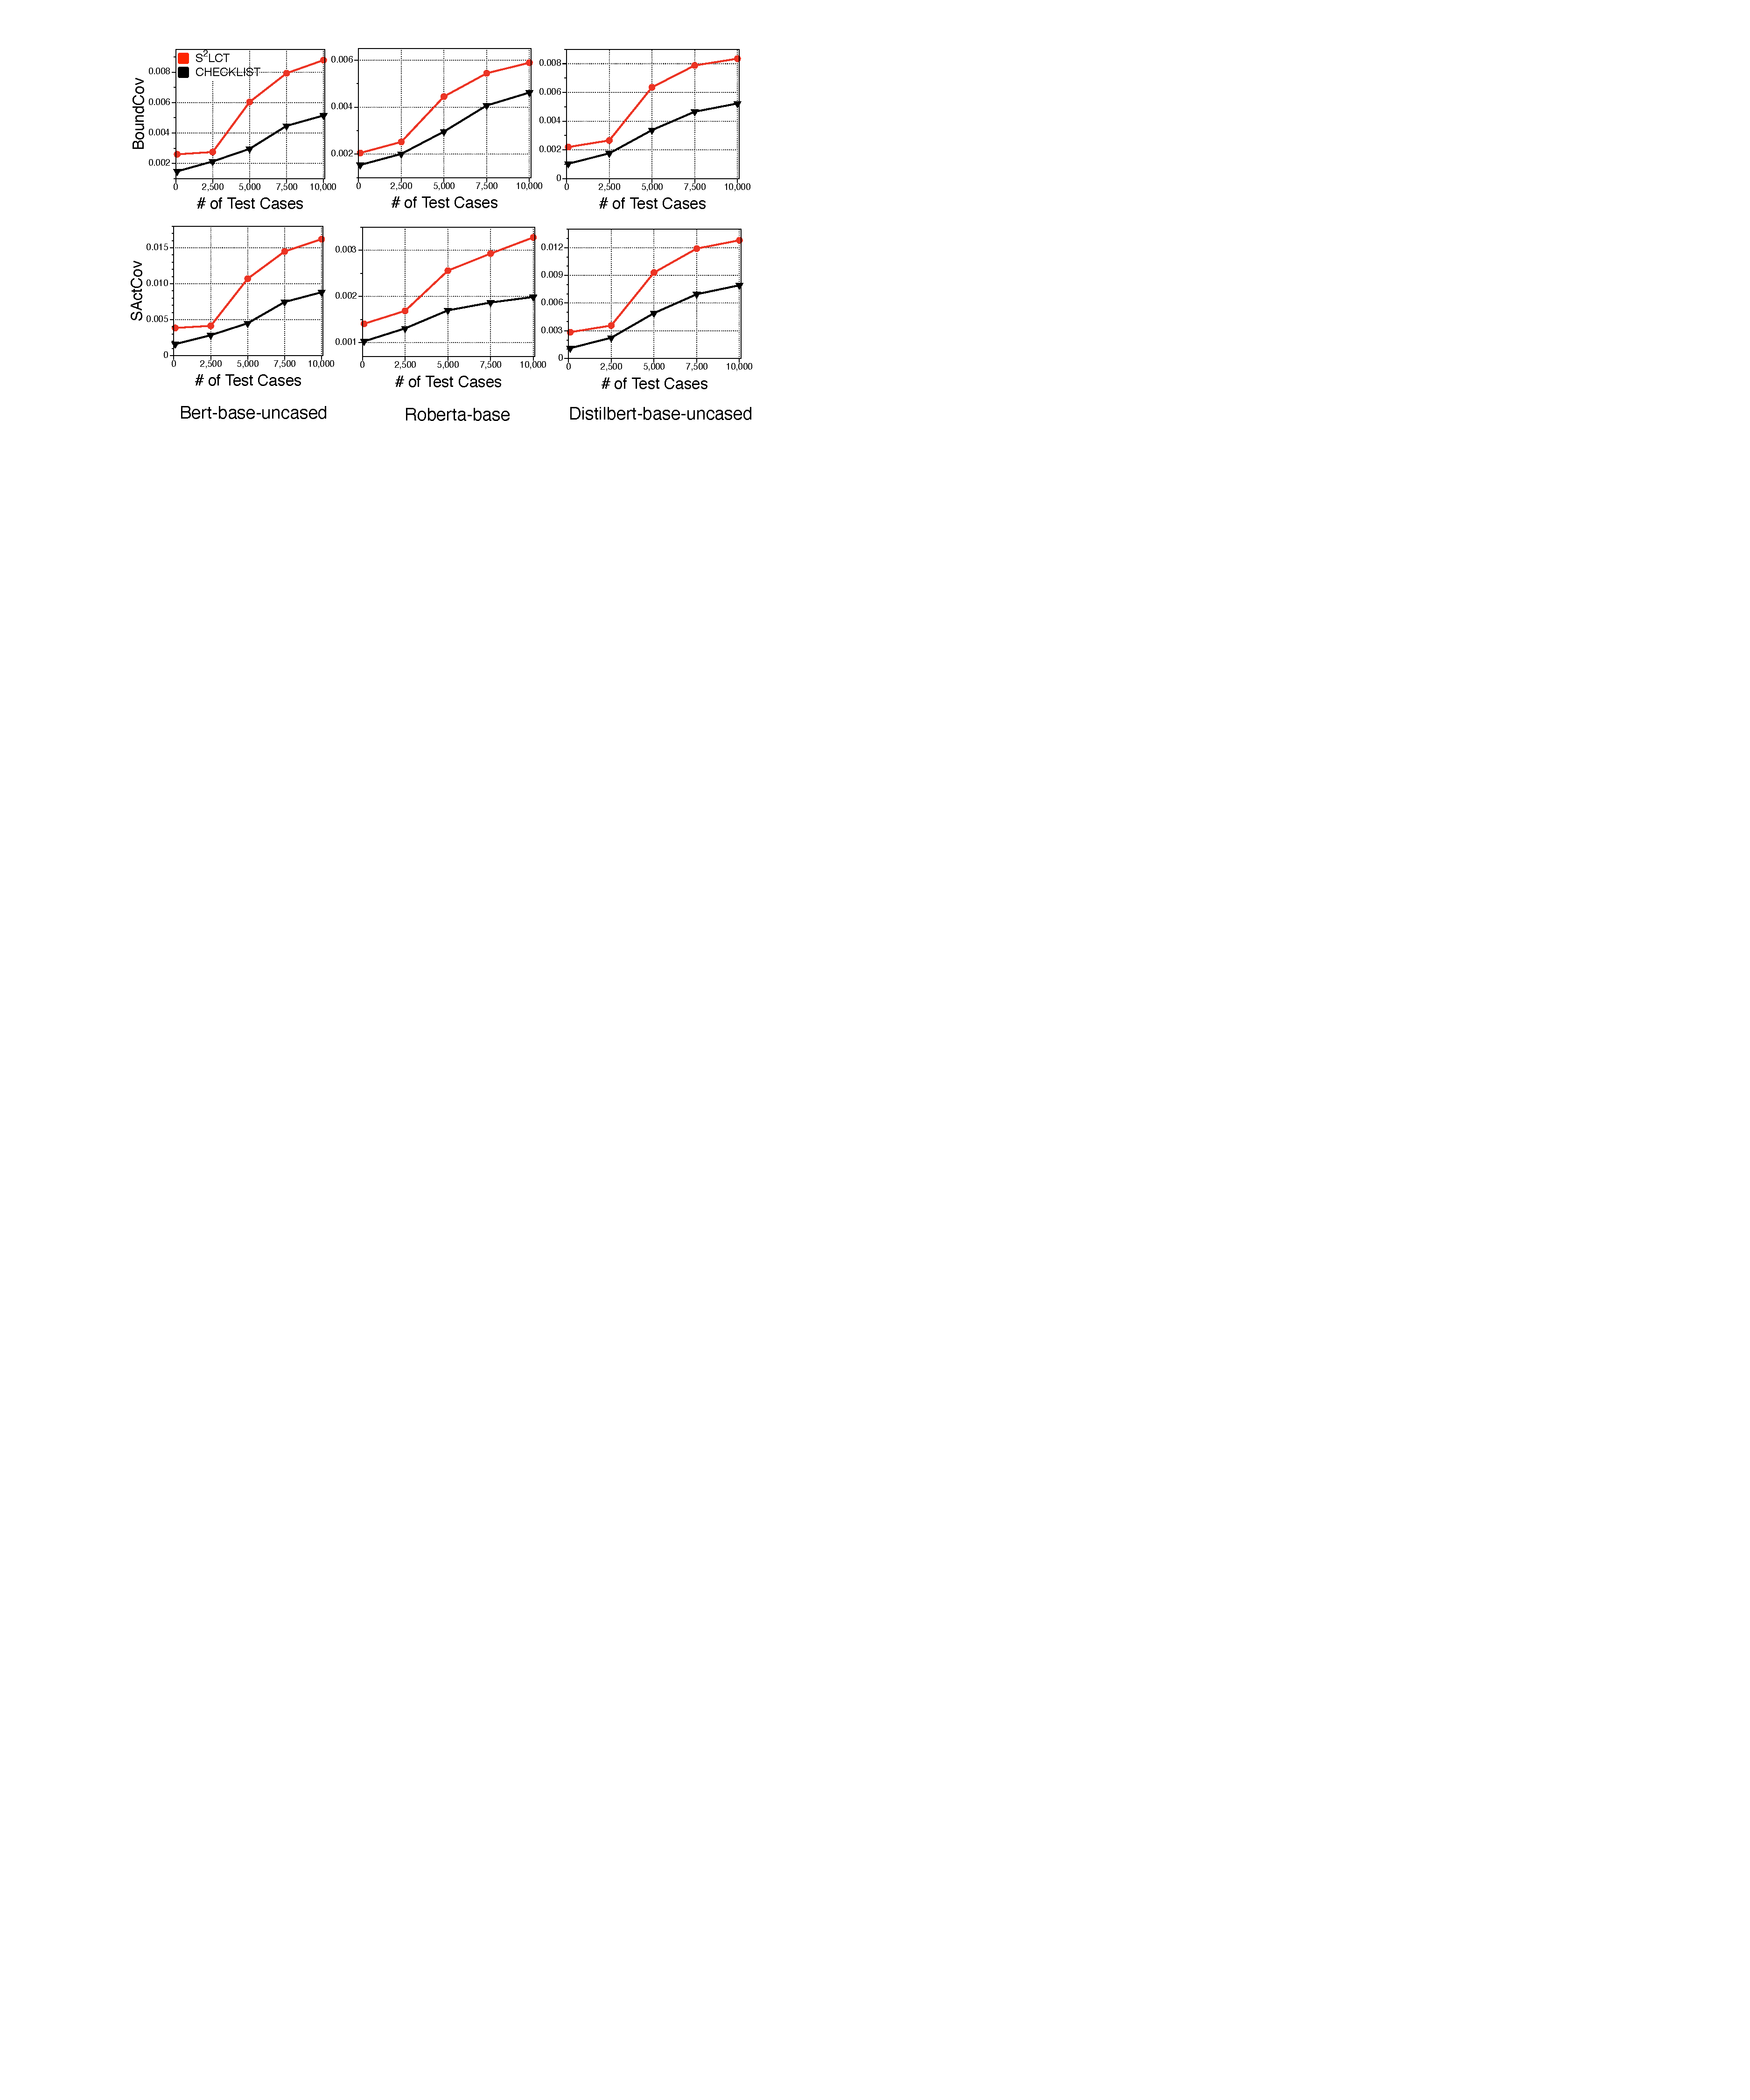
\includegraphics[width=0.5\textwidth]{figs/coverage.pdf}
    \vspace{-4mm}
    \caption{Coverage results of \tool and \Cklst test cases.}
    \label{fig:coverage}
\end{figure}

Next, Figure \ref{fig:coverage} shows the coverage results of \tool and \Cklst test cases. The red line represents \tool coverage and the black line represents \Cklst coverage. Each column in Figure \ref{fig:coverage} represents the results for one NLP model. The first row is the \textit{BoundCov} results and the second row is the \textit{SActCov} results.

We made three observations.
First, for \emph{all} experimental settings (i.e., NLP model and coverage metric), \tool achieves higher coverage than \Cklst. Recall that a higher coverage implies the test cases are more diverse and do not have a similar statistical distribution to the model training data. As a result, a test suite with greater coverage complements the model training data distribution (\ie holdout testing data) better.
For example, for the first NLP model under test, \tool can achieve a higher coverage than \Cklst with only half the number of test cases.
This result confirms that \tool can generate more diverse test cases to complement the holdout dataset for testing NLP models.

Second, as the number of test cases increases, the test suite can achieve better coverage. Such observation is intuitive. However, generating a more extensive test suite is not easy, particularly  for \Cklst, which is a manually template-based approach.

Third, for each NLP model, there is no fixed relationship between \textit{BoundCov} and \textit{SActCov}. In other words, while a test suite may produce higher \textit{BoundCov} for some models, the same test suite may get higher \textit{SActCov} for other NLP models.
Recall that \textit{BoundCov} measures both the upper and lower corner neurons and \textit{SActCov} measures only the upper corner neurons. 
Such observation implies that the upper and lower corner neurons are distributed unevenly, and measuring only one of them is not enough.

%\subsection{Explainability Case Study}

